\chapter{Complément sur la dérivation}

\section{Rappels sur la dérivation}

\begin{definition}[Nombre dérivé et tangente]
	Soit $f$ une fonction définie sur un intervalle $I$ et soit $x_A \in I$.
	\begin{itemize}
		\item Le \textbf{taux de variation} de $f$ entre $x_A$ et $x_A+h$ (avec $h \neq 0$) est le nombre :
		      \[
			      \dfrac{f(x_A+h)-f(x_A)}{h}
		      \]
		\item La fonction $f$ est dite \textbf{dérivable} en $x_A$ si la limite du taux de variation lorsque $h$ tend vers $0$ existe et est un nombre réel, appelé \textbf{nombre dérivé} de $f$ en $x_A$ et noté $f^\prime(x_A)$ :
		      \[
			      f^\prime(x_A) = \lim_{h \to 0} \dfrac{f(x_A+h)-f(x_A)}{h}
		      \]
		\item Géométriquement, $f^\prime(x_A)$ est le coefficient directeur de la \textbf{tangente} à $\Cf$ au point $A\coordl{x_A}{f(x_A)}$.

		      L'équation réduite de cette tangente est :
		      \[
			      y = f^\prime(x_A)(x-x_A) + f(x_A)
		      \]
	\end{itemize}

	\begin{center}
		\begin{tikzpicture}[>=Stealth, x=9mm, y=9mm]
			\clip (-1.5,-1.5) rectangle (7.5,6);
			\draw[->, thick] (-1,0) -- (7,0) node[below left] {$x$};
			\draw[->, thick] (0,-1) -- (0,5.5) node[below left] {$y$};
			\node[below left] at (0,0) {$0$};
			\draw[domain=0.3:5.8, smooth, variable=\x, line width=1.5pt, blue] plot ({\x}, {0.15*(\x)^2 + 0.5});
			\node[blue, above right] at (4.6, 5.0) {$\mathcal{C}_f$};
			\def\a{2.1}
			\pgfmathsetmacro{\fa}{0.15*(\a)^2 + 0.5}
			\pgfmathsetmacro{\fprime}{0.3*\a}
			\coordinate (A) at (\a, \fa);
			\draw[dashed, gray, thick] (A) -- (\a, 0) node[below, black] {$x_A$};
			\draw[dashed, gray, thick] (A) -- (0, \fa) node[left, black] {$f(x_A)$};
			\draw[domain=0.3:5.5, smooth, variable=\x, line width=1.2pt, red!80!black] plot ({\x}, {\fprime * (\x - \a) + \fa}) node[above right] {$T$};
			\draw[->, thick, green!50!black] (\a, \fa) -- (\a+2, \fa) node[midway, below, fill=white] {$1$};
			\draw[->, thick, green!50!black] (\a+2, \fa) -- (\a+2, {\fa + \fprime*2}) node[midway, right, fill=white] {$f^\prime(x_A)$};
			\fill[black] (A) circle (2pt) node[above left] {$A$};
		\end{tikzpicture}
	\end{center}\end{definition}

\begin{prop}[Lien entre dérivée et variations]
	Soit $f$ une fonction dérivable sur un intervalle $I$.
	\begin{itemize}
		\item Si $f^\prime(x) \geq 0$ pour tout $x \in I$, alors $f$ est \textbf{croissante} sur $I$.
		\item Si $f^\prime(x) \leq 0$ pour tout $x \in I$, alors $f$ est \textbf{décroissante} sur $I$.
		\item Si $f^\prime$ s'annule et change de signe en un réel $c \in I$, alors $f$ admet un \textbf{extremum local} en $c$.
	\end{itemize}
\end{prop}

\begin{ex}[Étude des variations d'une fonction]
	Soit $f$ la fonction définie sur $\R$ par $f(x) = 2x^2 - 8x + 1$.

	Sa fonction dérivée est donnée par $f'(x) = 4x - 8$.

	Résolvons $f'(x) > 0$ :
	\[
		\begin{array}{rcl}
			4x - 8 > 0 & \iff & 4x > 8 \\
			           & \iff & x > 2
		\end{array}
	\]

	On en déduit le tableau de variations de $f$ :

	\begin{center}
		\begin{tikzpicture}
			\tikzset{arrow style/.style={>=Stealth, line width=1.2pt, ->}}
			\tkzTabInit[lgt=1.5, espcl=3]{$x$ / 0.75, $f'(x)$ / 0.75, $f(x)$ / 1.5}{$-\infty$, $2$, $+\infty$}
			\tkzTabLine{, -, z, +, }
			\tkzTabVar{+ / , - / $-7$, + / }
		\end{tikzpicture}
	\end{center}

	On calcule la valeur minimale : $f(2) = 2(2)^2 - 8(2) + 1 = -7$
\end{ex}
\section{Compléments sur les dérivées usuelles}

\begin{prop}[Formules des dérivées usuelles]
	Le tableau ci-dessous récapitule et complète les dérivées des fonctions usuelles :
	\[
		\def\arraystretch{1.7}
		\begin{array}{|c|c|c|c|} \hline
			\ccg \text{Fonction : } f(x)       & \ccg\text{Ensemble de définition : } D_f & \ccg\text{Fonction dérivée : } f'(x) & \ccg\text{Ensemble de dérivabilité : } D_{f'} \\ \hline
			k \quad (k \in \R)                 & \R                                       & 0                                    & \R                                            \\ \hline
			x                                  & \R                                       & 1                                    & \R                                            \\ \hline
			x^n \quad (n \in \N^*)             & \R                                       & n x^{n-1}                            & \R                                            \\ \hline
			\rule[-4mm]{0mm}{11mm}\dfrac{1}{x} & \R^*                                     & \dfrac{-1}{x^2}                      & \R^*                                          \\ \hline
			\cos x                             & \R                                       & -\sin x                              & \R                                            \\ \hline
			\sin x                             & \R                                       & \cos x                               & \R                                            \\ \hline
		\end{array}
	\]
\end{prop}

\begin{ex}
	\nline
	\begin{itemize}
		\item Pour $f(x) = x^4$, on a $f'(x) = 4x^3$ sur $\R$.
		\item Pour $g(x) = \dfrac{1}{x}$, on a $g'(2) = \dfrac{-1}{2^2} = \dfrac{-1}{4}$.
	\end{itemize}
\end{ex}

\begin{ex}[Étude des variations d'une fonction avec un terme en $\tfrac{1}{x}$]
	Soit $f$ la fonction définie sur l'intervalle ouvert $]0; +\infty[$ par :
				\[
					f(x) = 2x + \frac{4}{x}
				\]

				Cette fonction est dérivable sur $]0; +\infty[$ comme somme de fonctions usuelles.

	\begin{enumerate}
		\item \textbf{Calcul de la fonction dérivée $f'(x)$ :}

		      En utilisant les formules de dérivation usuelles, on a :
		      \[
			      \def\arraystretch{1.8}
			      \begin{array}{rrccccl}
				           & f(x)  & = & 2x & + & 4 \times \left(\dfrac{1}{x}\right)    &                      \\
				      \iff & f'(x) & = & 2  & + & 4 \times \left(\dfrac{-1}{x^2}\right) & = 2 - \dfrac{4}{x^2}
			      \end{array}
		      \]

		      Pour étudier plus facilement le signe de cette dérivée, réduisons au même dénominateur :
		      \[
			      f'(x) = \frac{2x^2}{x^2} - \frac{4}{x^2} = \frac{2x^2 - 4}{x^2}
		      \]

		\item \textbf{Étude du signe de $f'(x)$ sur $\intoo{0}{+\infty}$ :}

		      Pour tout $x \in \intoo{0}{+\infty}$, le dénominateur $x^2$ est strictement positif.

		      Le signe de $f'(x)$ dépend donc uniquement de celui du numérateur, $2x^2 - 4$.

		      Recherchons quand la dérivée est positive :
		      \[
			      \begin{array}{rcl}
				      2x^2 - 4 > 0 & \iff & 2x^2 > 4                                                         \\
				                   & \iff & x^2 > 2                                                          \\
				                   & \iff & x > \sqrt{2} \quad (\text{car } x > 0 \text{ sur } ]0; +\infty[)
			      \end{array}
		      \]

		      La dérivée est donc négative avant $\sqrt{2}$ et positive après.

		\item \textbf{Tableau de variations de $f$ :}

		      On en déduit le tableau de variations de $f$ sur $]0; +\infty[$ :

		      \begin{center}
			      \begin{tikzpicture}
				      \tikzset{arrow style/.style={>=Stealth, line width=1.2pt, ->}}
				      \tkzTabInit[lgt=2, espcl=4]{$x$ / 0.75, $f'(x)$ / 0.75, $f(x)$ / 1.5}{0, $\sqrt{2}$, $+\infty$}
				      \tkzTabLine{d, -, z, +, }
				      \tkzTabVar{D+/$+\infty$, - / $4\sqrt{2}$, + / $+\infty$}
			      \end{tikzpicture}
		      \end{center}

		      \emph{Précisions :}
		      \begin{itemize}
			      \item La double barre en $0$ dans le tableau indique que $0$ est une valeur interdite (la fonction tend vers $+\infty$ lorsque $x$ se rapproche de $0$ par valeurs supérieures).
			      \item La valeur minimale atteinte en $x = \sqrt{2}$ est exacte :
			            \[
				            \def\arraystretch{1.8}
				            \begin{array}{rcll}
					            f\left(\sqrt{2}\right) & = & 2\sqrt{2} + \dfrac{4}{\sqrt{2}}\pa{\times\dfrac{\sqrt{2}}{\sqrt{2}}} &                             \\
					                                   & = & 2\sqrt{2} + 2\sqrt{2}                                                & =  4\sqrt{2} \approx 5{,}66
				            \end{array}
			            \]
		      \end{itemize}

		\item \textbf{Représentation :}
		      \begin{center}
			      \begin{center}
				      \begin{tikzpicture}[>=Stealth, x=16mm, y=8mm]
					      \draw[xstep=1, ystep=2, gray!40, thick, dashed] (0,0) grid (5.5, 8.5);
					      \draw[->, thick] (-0.8,0) -- (6,0) node[below left] {$x$};
					      \draw[->, thick] (0,-0.8) -- (0,9) node[below left] {$y$};
					      \node[below left] at (0,0) {$0$};
					      \foreach \x/\label in {
							      1/1, 1.414/\sqrt{2}, 2/2, 3/3, 4/4, 5/5} {
							      \draw (\x, 0.08) -- (\x, -0.08);
							      \node[below] at (\x, 0) {$\label$};
						      }
					      \foreach \y/\pos in {2/left, 4/left, 8/left} {
							      \draw (0.08, \y) -- (-0.08, \y);
							      \node[\pos] at (0, \y) {$\y$};
						      }
					      \draw (0.08, 6) -- (-0.08, 6);
					      \node[left] at (0, 5.656) {$4\sqrt{2}$};
					      \coordinate (M) at (1.414, 5.656);
					      \node[below right, red, fill=white] at (M) {$\text{Minimum } \left(\sqrt{2}\,;\,4\sqrt{2}\right)$};
					      \node[blue, above right, fill=white] at (4, 8) {$\mathcal{C}_f : y = 2x + \dfrac{4}{x}$};
					      \draw[domain=0.5:4.2, smooth, variable=\x, ultra thick, blue] plot ({\x}, {2*\x + 4/\x});
					      \fill[red] (M) circle (2.5pt);
					      \draw[dashed, red, very thick] (1.414, 0) -- (M);
					      \draw[dashed, red, very thick] (0, 5.656) -- (M);
				      \end{tikzpicture}
			      \end{center}
		      \end{center}

	\end{enumerate}
\end{ex}

\section{Compléments sur les opérations sur les fonctions dérivables}

\subsection{Produit de deux fonctions}

\begin{prop}[Dérivée d'un produit]
	Soient $u$ et $v$ deux fonctions définies et dérivables sur un même intervalle $I$.

	Alors la fonction produit $u \times v$ (notée $uv$) est dérivable sur $I$ et :
	\[
		(uv)' = u'v + uv'
	\]
\end{prop}

\begin{attention}
	La dérivée d'un produit \textbf{n'est pas} le produit des dérivées : $(uv)' \neq u' \times v'$.
\end{attention}

\begin{methode}[Calculer la dérivée d'un produit]
	Pour dériver une fonction de la forme $f(x) = u(x)\times v(x)$ :
	\begin{enumerate}
		\item Identifier clairement les fonctions $u(x)$ et $v(x)$.
		\item Calculer leurs dérivées respectives $u'(x)$ et $v'(x)$.
		\item Appliquer la formule $f'(x) = u'(x)v(x) + u(x)v'(x)$.
		\item Développer et réduire l'expression obtenue.
	\end{enumerate}
\end{methode}

\begin{ex}
	Soit $f$ la fonction définie sur $\R$ par $f(x) = (3x^2 + 4x)(5x - 1)$.

	La fonction $f$ est sous la forme $u \times v$ avec :
	\begin{itemize}
		\item $u(x) = 3x^2 + 4x \quad\Rarr\quad u'(x) = 6x + 4$
		\item $v(x) = 5x - 1 \quad\Rarr\quad v'(x) = 5$
	\end{itemize}

	En appliquant la formule de la dérivée d'un produit :
	\[
		\def\arraystretch{1.5}
		\begin{array}{rcl}
			f'(x) & = & u'(x)v(x) + u(x)v'(x)                                  \\
			      & = & (6x + 4)(5x - 1) + (3x^2 + 4x) \times 5                \\
			      & = & (30x^2 - 6x + 20x - 4) + (15x^2 + 20x)                 \\
			      & = & 30x^2 + 14x - 4 + 15x^2 + 20x \qquad = 45x^2 + 34x - 4
		\end{array}
	\]
\end{ex}

\subsection{Inverse d'une fonction}

\begin{prop}[Dérivée de l'inverse]
	Soit $u$ une fonction définie et dérivable sur un intervalle $I$, telle que $u(x) \neq 0$ pour tout $x \in I$.

	Alors la fonction inverse $\dfrac{1}{u}$ est dérivable sur $I$ et :
	\[
		\pa{\dfrac{1}{u}}' = \dfrac{-u'}{u^2}
	\]
\end{prop}

\begin{ex}
	Soit $g$ la fonction définie sur $\R$ par $g(x) = \dfrac{1}{2x^2 + 5x}$.

	La fonction $g$ est de la forme $\dfrac{1}{u}$ avec $u(x) = 2x^2 + 5x$.

	On a $u'(x) = 4x + 5$.

	Pour tout $x$ tel que $2x^2 + 5x \neq 0$ :
	\[
		g'(x) = \dfrac{-u'(x)}{(u(x))^2} = \dfrac{-4x + 5}{(2x^2 + 5x)^2}
	\]
\end{ex}

\subsection{Quotient de deux fonctions}

\begin{prop}[Dérivée d'un quotient]
	Soient $u$ et $v$ deux fonctions définies et dérivables sur un intervalle $I$, avec $v(x) \neq 0$ pour tout $x \in I$.

	Alors la fonction quotient $\dfrac{u}{v}$ est dérivable sur $I$ et :
	\[
		\pa{\dfrac{u}{v}}' = \dfrac{u'v - uv'}{v^2}
	\]
\end{prop}

\begin{erreur}
	Attention au signe moins au numérateur ! Ne pas confondre $u'v - uv'$ avec $uv' - u'v$.

	De plus, le dénominateur est $v^2$ et n'est jamais dérivé.
\end{erreur}

\begin{methode}[Calculer la dérivée d'un quotient]
	Soit à dériver $h(x) = \dfrac{x}{x^3 - 1}$ sur l'intervalle $\intoo{-\infty}{1} \cup \intoo{1}{+\infty}$.

	\begin{enumerate}
		\item On pose $u(x) = x \quad\Rarr\quad u'(x) = 1$.
		\item On pose $v(x) = x^3 - 1 \quad\Rarr\quad v'(x) = 3x^2$.
		\item On applique la formule de dérivation du quotient :
		      \[
			      \def\arraystretch{2}
			      \begin{array}{rcll}
				      h'(x) & = & \dfrac{u'(x)v(x) - u(x)v'(x)}{(v(x))^2}                   &                                   \\
				            & = & \dfrac{1 \times (x^3 - 1) - x \times (3x^2)}{(x^3 - 1)^2} &                                   \\
				            & = & \dfrac{x^3 - 1 - 3x^3}{(x^3 - 1)^2}                       & =  \dfrac{-2x^3 - 1}{(x^3 - 1)^2}
			      \end{array}
		      \]
	\end{enumerate}
\end{methode}

\begin{ex}[Étude d'une fonction rationnelle (quotient)]
	Soit $f$ la fonction définie sur l'ensemble $I = \intoo{2}{+\infty}$ par :
	\[
		f(x) = \frac{x^2 - 3}{2 - x} + 10
	\]

	\begin{enumerate}
		\item \textbf{Calcul de la fonction dérivée $f'(x)$ :}

		      La fonction $f$ est de la forme $\dfrac{u}{v} + k$ avec :
		      \begin{itemize}
			      \item $u(x) = x^2 - 3 \quad\Rarr\quad u'(x) = 2x$
			      \item $v(x) = 2 - x \quad\Rarr\quad v'(x) = -1$
		      \end{itemize}

		      En appliquant la formule de dérivation d'un quotient $\pa{\dfrac{u}{v}}' = \dfrac{u'v - uv'}{v^2}$ et sachant que la dérivée de la constante $10$ est nulle :
		      \[
			      \def\arraystretch{2}
			      \begin{array}{rcll}
				      f'(x) & = & \dfrac{2x(2 - x) - (x^2 - 3) \times (-1)}{(2 - x)^2} + 0 &                                    \\
				            & = & \dfrac{4x - 2x^2 + x^2 - 3}{(2 - x)^2}                   & = \dfrac{-x^2 + 4x - 3}{(2 - x)^2}
			      \end{array}
		      \]

		\item \textbf{Étude du signe de $f'(x)$ sur $I = \intoo{2}{+\infty}$ :}

		      Pour tout $x \in \intoo{2}{+\infty}$, le dénominateur $(2 - x)^2$ est strictement positif.

		      Le signe de $f'(x)$ dépend donc uniquement du signe du numérateur, $-x^2 + 4x - 3$.

		      Recherchons les racines du trinôme $-x^2 + 4x - 3$ :

		      Le discriminant vaut $\Delta = 4^2 - 4 \times (-1) \times (-3) = 16 - 12 = 4 = 2^2$.

		      Puisque $\Delta > 0$, le trinôme admet deux racines distinctes :
		      \[
			      x_1 = \frac{-4 + 2}{-2} = 1 \quad\text{et}\quad x_2 = \frac{-4 - 2}{-2} = 3
		      \]

		      Remarquons que la racine $x_1 = 1$ est hors de l'intervalle d'étude $\intoo{2}{+\infty}$.

		      Seule la racine $x_2 = 3$ appartient à l'intervalle $\intoo{2}{+\infty}$.

		      Le coefficient de $x^2$ étant négatif ($-1 < 0$), le trinôme est positif entre $1$ et $3$, et négatif à l'extérieur.

		      Sur l'intervalle $\intoo{2}{+\infty}$ :
		      \begin{itemize}
			      \item Pour $x \in \intoo{2}{3}$, $f'(x) \geq 0$.
			      \item Pour $x \in \intoo{3}{+\infty}$, $f'(x) \leq 0$.
		      \end{itemize}

		\item \textbf{Tableau de variations de $f$ :}

		      \begin{center}
			      \begin{tikzpicture}
				      \tikzset{arrow style/.style={>=Stealth, line width=1.2pt, ->}}
				      \tkzTabInit[lgt=2.5, espcl=4]{$x$ / 0.75, $f'(x)$ / 0.75, $f(x)$ / 1.5}{$2$, $3$, $+\infty$}
				      \tkzTabLine{d, +, z, -, }
				      \tkzTabVar{D-/$-\infty$, + / $4$, - / $-\infty$}
			      \end{tikzpicture}
		      \end{center}

		      \emph{Précision :} Le maximum est atteint en $x = 3$ et vaut $f(3) = \dfrac{3^2 - 3}{2 - 3} + 10 = -6 + 10 = 4$.

		\item \textbf{Représentation :}

		      \begin{center}
			      \begin{tikzpicture}[>=Stealth, x=15mm, y=6mm]
				      \draw[xstep=1, ystep=2, gray!40, dashed] (0, -5) grid (6.5, 6);
				      \draw[->, thick] (-0.5,0) -- (6.8,0) node[below left] {$x$};
				      \draw[->, thick] (0,-5) -- (0,7.5) node[right] {$y$};
				      \node[below left] at (2,0) {$2$};
				      \foreach \x/\label in {1/1, 3/3, 4/4, 5/5, 6/6} {
						      \draw (\x, 0.08) -- (\x, -0.08);
						      \node[below] at (\x, 0) {$\label$};
					      }
				      \draw (2, 0.08) -- (2, -0.08); % Graduation 2
				      \foreach \y/\pos in {-4/left, -2/left, 2/left, 4/left, 6/left} {
						      \draw (0.08, \y) -- (-0.08, \y);
						      \node[\pos] at (0, \y) {$\y$};
					      }
				      \draw[thick, red!70!black, dashed] (2,-5) -- (2,6.5) node[above, fill=white] {Asymptote $x = 2$};
				      \coordinate (M) at (3, 4);
				      \node[above right, red, fill=white] at (M) {$\text{Maximum } (3\,;\,4)$};
				      \node[blue, fill=white] at (5, 2) {$\Cf$};
				      \draw[domain=2.1:6.2, smooth, samples=100, variable=\x, ultra thick, blue] plot ({\x}, {(\x^2 - 3)/(2 - \x) + 10});
				      \fill[red] (M) circle (2.5pt);
				      \draw[dashed, red, very thick] (3, 0) -- (M);
				      \draw[dashed, red, very thick] (0, 4) -- (M);
			      \end{tikzpicture}
		      \end{center}
	\end{enumerate}
\end{ex}

\section{Dérivées de fonctions composées particulières}

\subsection{Composition avec des fonctions affines}

\begin{prop}[Dérivée de $f(ax+b)$]
	Soit $f$ une fonction dérivable sur un intervalle $J$, et soient $a$ et $b$ deux réels.

	Pour tout $x$ tel que $ax+b \in J$, la fonction $g : x \mapsto f(ax+b)$ est dérivable et :
	\[
		g'(x) = a f'(ax+b)
	\]
\end{prop}

\begin{ex}
	Soit $k(x) = (4x - 3)^3$.

	On pose $f(X) = X^3$ et donc $k(x)=f(4x-3)$

	Ici $a = 4$ et $b = -3$ et $f'(X) = 3X^2$.

	On obtient :
	\[
		\begin{array}{rcl}
			k'(x) & = & 4\times f'(4x - 3)   \\
			      & = & 4 \times 3(4x - 3)^2 \\
			      & = & 12(4x - 3)^2
		\end{array}
	\]
\end{ex}

\subsection{Fonctions sinusoïdales composées}

\begin{prop}[Dérivées des fonctions trigonométriques composées]
	Soient $A$, $\omega$ et $\varphi$ trois réels constants.
	\begin{itemize}
		\item La fonction $t \mapsto A \cos(\omega t + \varphi)$ a pour fonction dérivée :
		      \[
			      t \mapsto -A\omega \sin(\omega t + \varphi)
		      \]
		\item La fonction $t \mapsto A \sin(\omega t + \varphi)$ a pour fonction dérivée :
		      \[
			      t \mapsto A\omega \cos(\omega t + \varphi)
		      \]
	\end{itemize}
\end{prop}

\begin{ex}[Calculer des dérivées de fonctions composées trigonométriques]
	\nline
	\begin{enumerate}
		\item Soit $f(t) = 3 \cos(2t + \pi)$.

		      En identifiant $A = 3$, $\omega = 2$ et $\varphi = \pi$ :
		      \[
			      f'(t) = -3 \times 2 \sin(2t + \pi) = -6 \sin(2t + \pi)
		      \]
		\item Soit $g(t) = -4 \sin\pa{-3t - \dfrac{\pi}{4}}$.

		      En identifiant $A = -4$, $\omega = -3$ et $\varphi = \dfrac{-\pi}{4}$ :
		      \[
			      g'(t) = -4 \times (-3) \cos\pa{-3t - \dfrac{\pi}{4}} = 12 \cos\pa{-3t - \dfrac{\pi}{4}}
		      \]
	\end{enumerate}
\end{ex}
